\part{Cálculos manuales}

Esta sección tiene como objetivo modelar una ataguía mediante el empleo de redes de flujo y líneas equipotenciales graficadas a través de \textit{Python}. De esta manera, se busca calcular factores como el caudal de infiltración, la presión de poros a lo largo de la ataguía, la estabilidad, la falla por licuefacción y el factor de seguridad. Todos estos cálculos fueron realizados con \textit{Python}, lo que permitió efectuar un análisis más exhaustivo y preciso en los distintos casos.

\section{Teoría}

A continuación, se presentará la teoría utilizada para el cálculo en esta sección.

\subsection{Líneas de flujo}
Las líneas de flujo representan las trayectorias que siguen las partículas de agua al moverse a través de un medio poroso. En un diagrama de flujo, estas líneas son perpendiculares a las líneas equipotenciales y muestran la dirección del flujo subterráneo o de infiltración. En estructuras como las ataguías, las líneas de flujo se usan para predecir el comportamiento del agua alrededor y debajo de la estructura, ayudando a diseñar sistemas eficaces de control de agua \citep{structville}.

\subsection{Líneas equipotenciales}
Las líneas equipotenciales representan ubicaciones con igual carga hidráulica, lo que significa que no se identifica diferencia de energía a lo largo de ellas. En problemas de flujo de agua subterránea, como los relacionados con las ataguías, estas líneas ayudan a visualizar la distribución de la energía potencial dentro del agua. Así, fundamentales para determinar el caudal de agua y asegurar que esta no desestabilice estructuras como los diques o presas \citep{structville}.

\subsection{Caudal de infiltración}
El caudal de infiltración es el flujo de agua que penetra a través del suelo debido a la diferencia de presión entre el nivel de agua dentro y fuera de la ataguía. La tasa de infiltración está condicionada por la permeabilidad del suelo y la diferencia de carga hidráulica. Para calcular el caudal de infiltración, se utiliza la fórmula (\ref{eq:caudal_infiltracion}) \citep{stability_cofferdam_2024}:

\begin{equation}
    Q = k \cdot \frac{\Delta H}{N_{f}} \cdot N_{d}
    \label{eq:caudal_infiltracion}
\end{equation}

Donde:
\begin{itemize}
    \item $Q$ = Caudal de infiltración
    \item $k$ = Coeficiente de permeabilidad
    \item $\Delta H$ = Diferencia de carga hidráulica
    \item $N_{f}$ = Cantidad de canales de flujo
    \item $N_{d}$ = Cantidad de canales equipotenciales
\end{itemize}

\subsection{Presión de poros}
La presión de poros es la fuerza que el agua ejerce dentro de los poros de un material, como el suelo o la roca. Juega un papel crucial en la construcción en terrenos con agua o alto nivel freático, ya que una presión de poros excesiva puede reducir el esfuerzo efectivo en el suelo. Lo anterior podría ocasionar problemas como la licuefacción, en el cual el suelo pierde firmeza, o la formación de tuberías subterráneas. En las ataguías, la presión de poros es un factor clave, ya que afecta la estabilidad del terreno que rodea la estructura. Para calcular la presión de poros, se utiliza la siguiente fórmula \citep{jeas}.

\begin{equation}
    u = \gamma \cdot h
    \label{eq:presion_poros}
\end{equation}

Donde:
\begin{itemize}
    \item $u$ = Presión de poros
    \item $\gamma$ = Peso específico del agua
    \item $h$ = Profundidad del agua
\end{itemize}

\subsection{Gradiente hidráulico}
El gradiente hidráulico equivale a el cambio de la carga hidráulica por unidad de distancia en la dirección del flujo. Constituye un factor crucial para determinar el flujo de agua a través de suelos. En el diseño de ataguías, el gradiente hidráulico ayuda a predecir problemas como la licuefacción, donde los gradientes elevados pueden erosionar el suelo y causar fallos estructurales. Este se calcula con la fórmula (\ref{eq:gradiente_hidraulico}) \citep{budhu_soil_2010}.

\begin{equation}
    i = \frac{\Delta h}{\Delta L}
    \label{eq:gradiente_hidraulico}
\end{equation}

Donde:
\begin{itemize}
    \item $i$ = Gradiente hidráulico
    \item $\Delta h$ = Cambio de carga hidráulica
    \item $\Delta L$ = Distancia en la dirección del flujo
\end{itemize}

\subsubsection{Licuefacción}
La licuefacción se produce cuando se excede el gradiente hidráulico crítico (\ref{eq:gradiente_critico}), lo que provoca que el suelo pierda su capacidad de soporte y se comporte como un líquido. En el diseño de ataguías, la licuefacción es un problema grave, ya que puede causar el colapso de la estructura y daños significativos a la infraestructura circundante \citep{budhu_soil_2010}.

\begin{equation}
    i_{critico} = \frac{\Delta h}{L_{min}}
    \label{eq:gradiente_critico}
\end{equation}

\subsection{Presión en una ataguía}
La presión dentro y alrededor de una ataguía es resultado tanto del nivel de agua como de las condiciones del suelo. Debido a estos, el diseño de una ataguía implica calcular la caída de carga potencial, la presión de poros y el gradiente hidráulico, lo que permite predecir si la estructura soportará las presiones del agua y del suelo que actúan sobre ella. Las redes de flujo se utilizan para evaluar estas presiones y estimar la infiltración de agua a través de la cimentación \citep{sivakugan2005}.

\section{Resultados}

\subsection{Diagramas Escala 1:200}

\begin{figure}[H]
    \centering
    \begin{minipage}{0.32\textwidth}
        \centering
        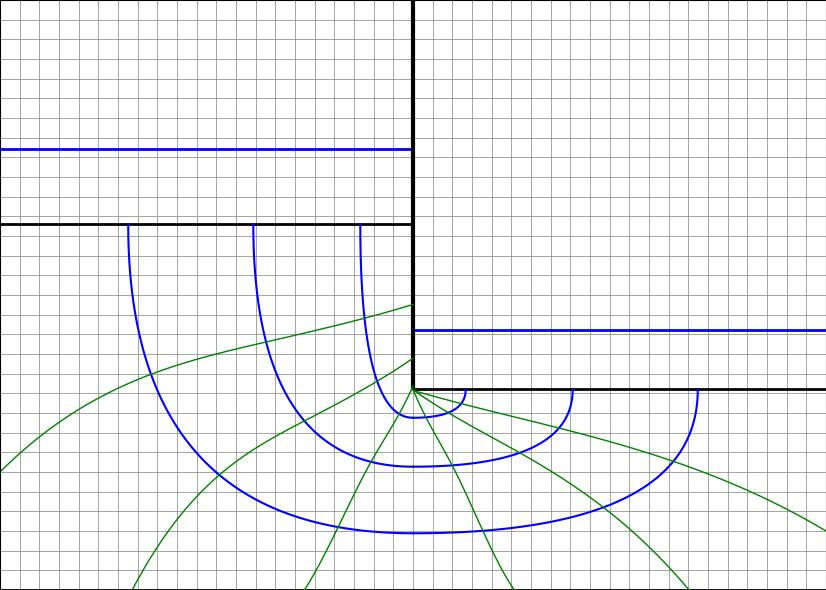
\includegraphics[width=\textwidth]{GRAFICOS/caso_1.jpg}
        \caption{Caso 1}
        \text{Fuente: Elaboración propia}
        \label{fig:caso_1}
    \end{minipage}
    \begin{minipage}{0.32\textwidth}
        \centering
        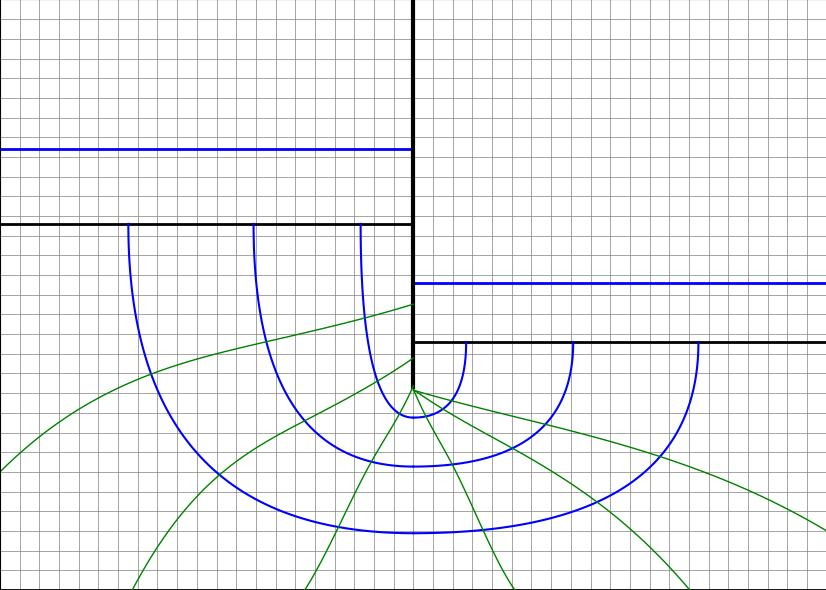
\includegraphics[width=\textwidth]{GRAFICOS/caso_2.jpg}
        \caption{Caso 2}
        \text{Fuente: Elaboración propia}
        \label{fig:caso_2}
    \end{minipage}
    \begin{minipage}{0.32\textwidth}
        \centering
        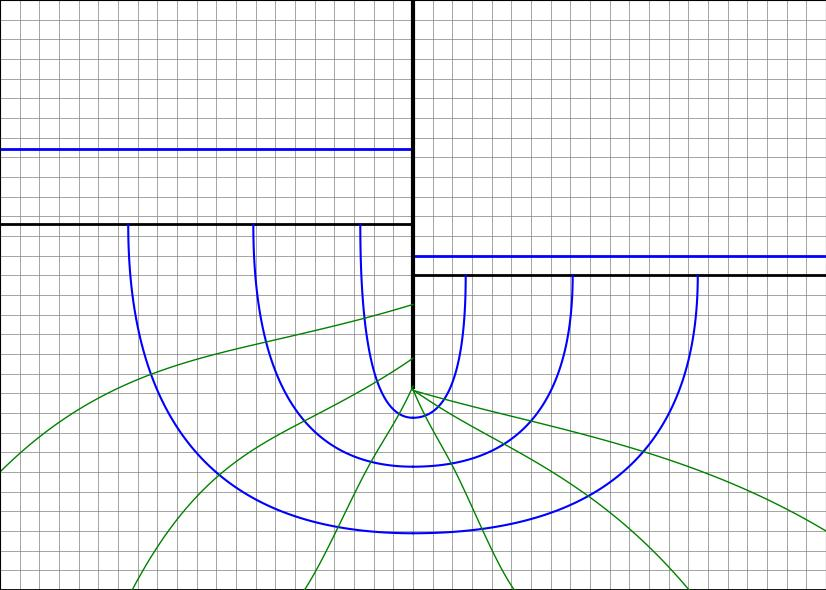
\includegraphics[width=\textwidth]{GRAFICOS/caso_3.jpg}
        \caption{Caso 3}
        \text{Fuente: Elaboración propia}
        \label{fig:caso_3}
    \end{minipage}
\end{figure}

Con el fin de visualizar los tres casos de ataguías, se graficaron los diagramas a escala 1:200. En estos, se pueden observar las líneas de flujo (azules) y equipotenciales (verdes), las cuales permiten analizar el comportamiento del agua alrededor de la estructura. Es importante señalar que, en el caso 1, el agua recorre una menor distancia para atravesar la barrera, lo que resulta en un mayor volumen de infiltración. Por otro lado, el caso 3 presenta una mayor longitud de línea de flujo, lo que genera una menor cantidad de infiltración.

\subsection{Presión de poros}
Para calcular la presión de poros en cada caso, se utilizó la fórmula (\ref{eq:presion_poros}). 

\subsubsection{Distribución de presiones}

\begin{figure}[H]
    \centering
    \begin{minipage}{0.32\textwidth}
        \centering
        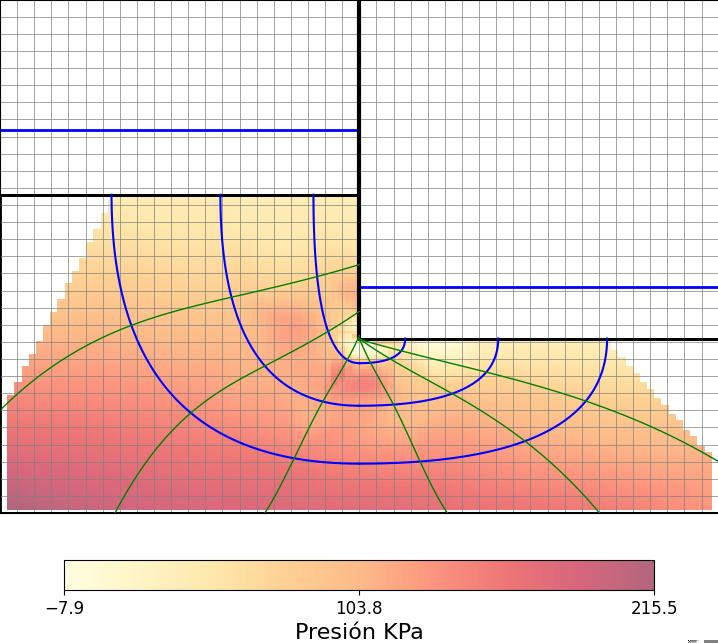
\includegraphics[width=\textwidth]{GRAFICOS/caso_1_presion_poros.jpg}
        \caption{Caso 1 Presión de Poros}
        \text{Fuente: Elaboración propia}
        \label{fig:caso_1_presion_poros}
    \end{minipage}
    \begin{minipage}{0.32\textwidth}
        \centering
        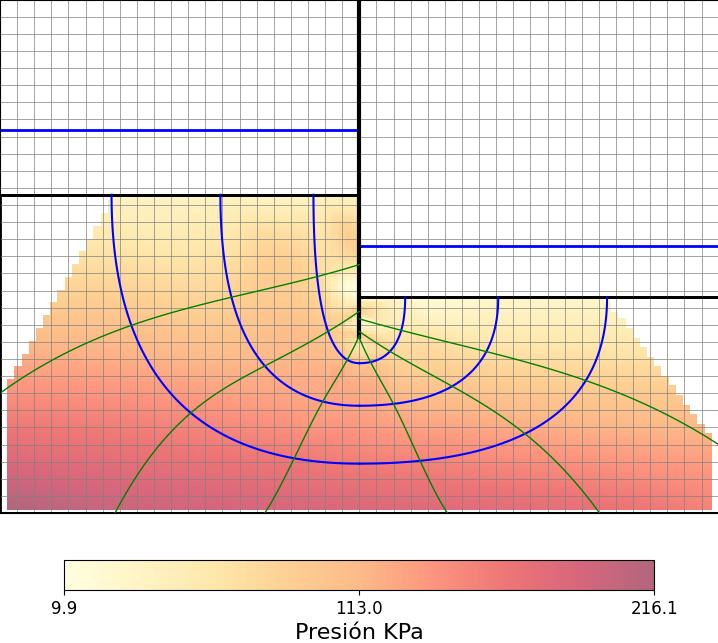
\includegraphics[width=\textwidth]{GRAFICOS/caso_2_presion_poros.jpg}
        \caption{Caso 2 Presión de Poros}
        \text{Fuente: Elaboración propia}
        \label{fig:caso_2_presion_poros}
    \end{minipage}
    \begin{minipage}{0.32\textwidth}
        \centering
        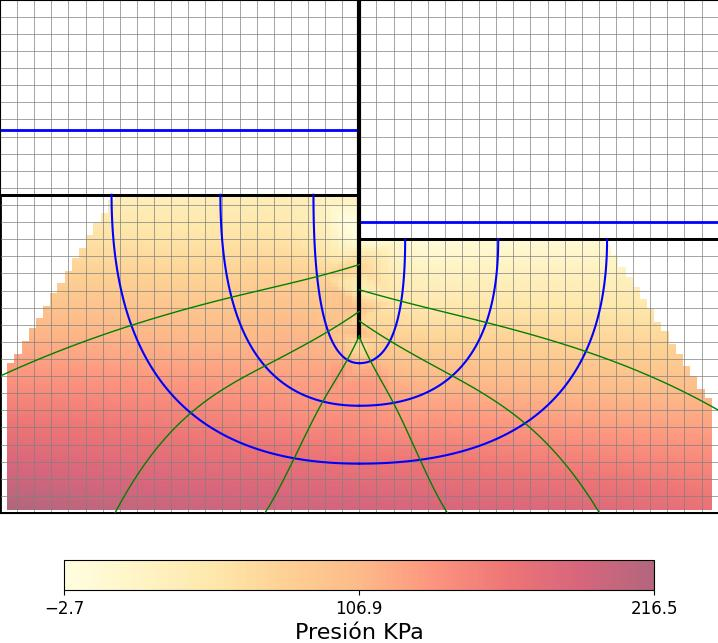
\includegraphics[width=\textwidth]{GRAFICOS/caso_3_presion_poros.jpg}
        \caption{Caso 3 Presión de Poros}
        \text{Fuente: Elaboración propia}
        \label{fig:caso_3_presion_poros}
    \end{minipage}
\end{figure}

Como se puede observar, para la figura \ref{fig:caso_1_presion_poros}, en la parte inferior de la ataguía se presenta una mayor presión de poros que en los otros dos casos, esto genera un mayor gradiente hidráulico, lo que podría producir licuefacción. Por otro lado, en las figuras \ref{fig:caso_2_presion_poros} y \ref{fig:caso_3_presion_poros}, se observa que la presión de poros es menor en la parte inferior de la ataguía, lo que se traduce en una menor presión hidráulica y mayor estabilidad.

\subsubsection{Presiones totales}

\begin{figure}[H]
    \centering
    \begin{minipage}{0.32\textwidth}
        \centering
        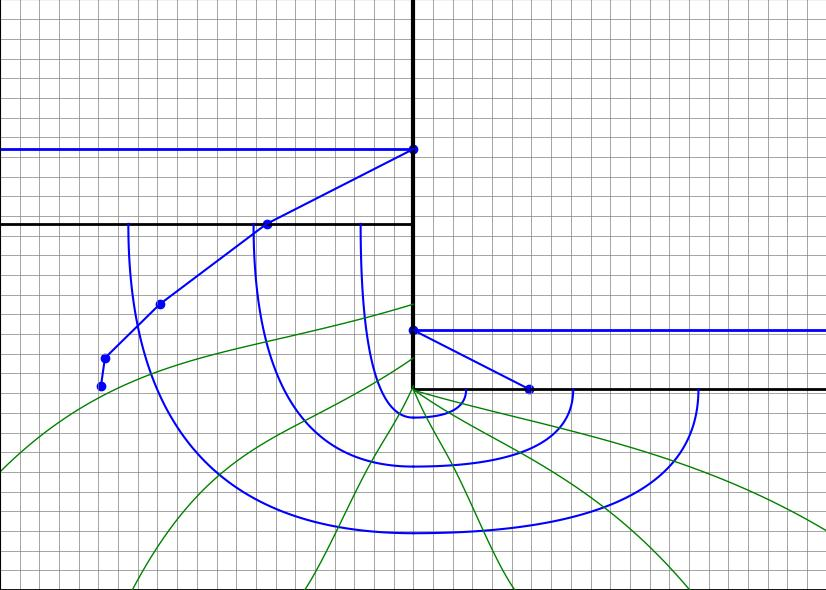
\includegraphics[width=\textwidth]{GRAFICOS/caso_1_presion_ataguia_total.jpg}
        \caption{Caso 1 Presión ataguía total}
        \text{Fuente: Elaboración propia}
        \label{fig:caso_1_presion_ataguia_total}
    \end{minipage}
    \begin{minipage}{0.32\textwidth}
        \centering
        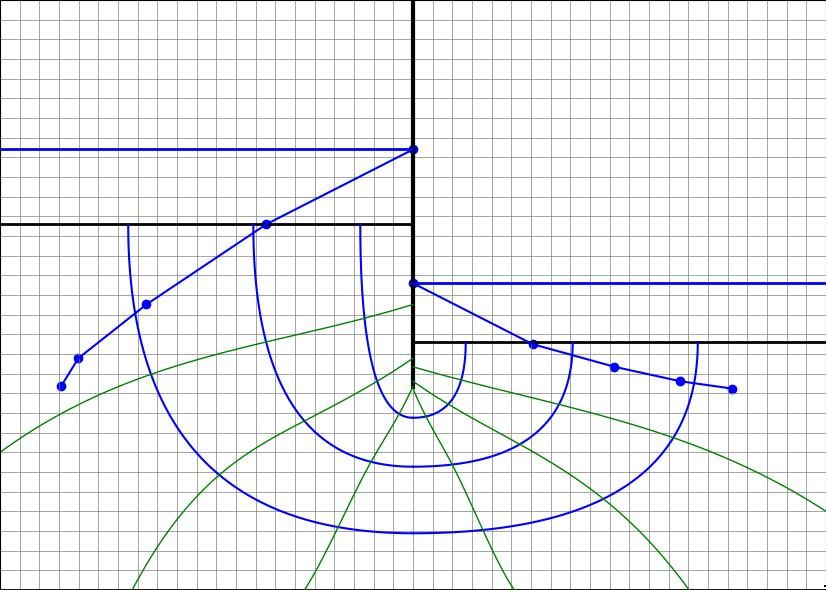
\includegraphics[width=\textwidth]{GRAFICOS/caso_2_presion_ataguia_total.jpg}
        \caption{Caso 2 Presión ataguía total}
        \text{Fuente: Elaboración propia}
        \label{fig:caso_2_presion_ataguia_total}
    \end{minipage}
    \begin{minipage}{0.32\textwidth}
        \centering
        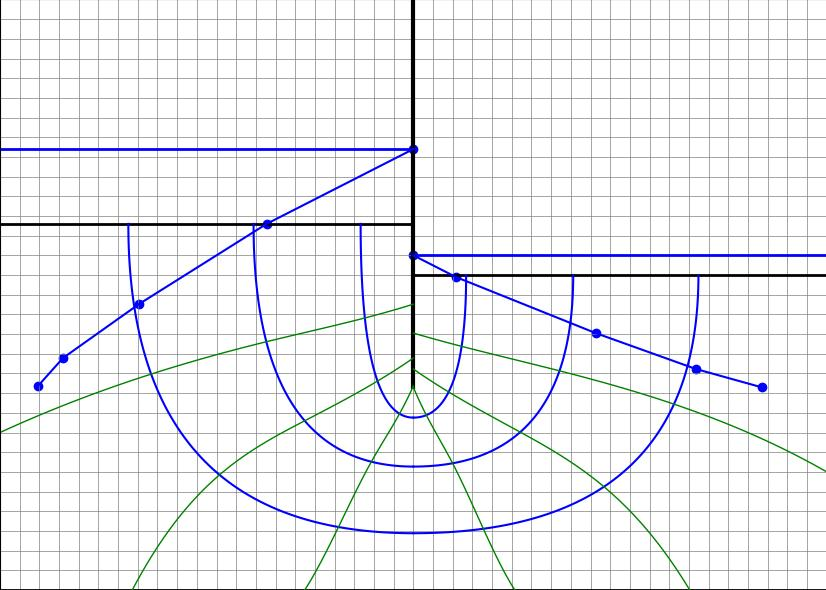
\includegraphics[width=\textwidth]{GRAFICOS/caso_3_presion_ataguia_total.jpg}
        \caption{Caso 3 Presión ataguía total}
        \text{Fuente: Elaboración propia}
        \label{fig:caso_3_presion_ataguia_total}
    \end{minipage}
\end{figure}

En los diagramas de presión total, se puede observar que, en todos los casos, la fuerza ejercida en la parte derecha de la ataguía es similar. Sin embargo, en la parte izquierda, a medida que aumenta el nivel del suelo, también lo hace la magnitud de la carga. Esto se aprecia claramente en la figura \ref{fig:caso_1_presion_ataguia_total}, donde la intensidad en el lado derecho es baja, mientras que en la figura \ref{fig:caso_3_presion_ataguia_total}, los valores son mayores. Estos efectos se reflejan directamente en las presiones efectivas.


\subsubsection{Presiones efectivas}

Con el fin de apreciar mejor el efecto de las presiones en la ataguía, se diagramaron las presiones efectivas. Estas se calculan restando la presión en el lado derecho de la ataguía con la del lado izquierdo.

\begin{figure}[H]
    \centering
    \begin{minipage}{0.32\textwidth}
        \centering
        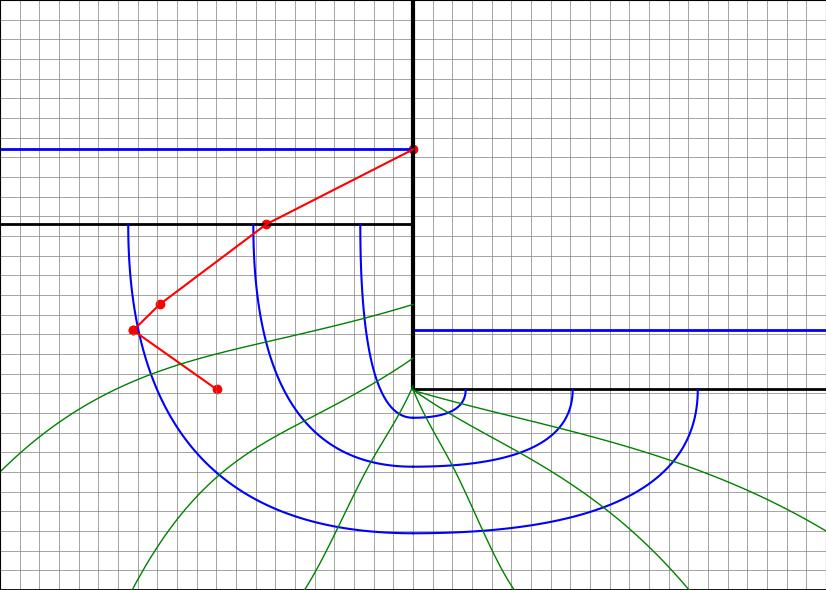
\includegraphics[width=\textwidth]{GRAFICOS/caso_1_presion_ataguia_neta.jpg}
        \caption{Caso 1 Presión ataguía neta}
        \text{Fuente: Elaboración propia}
        \label{fig:caso_1_presion_ataguia_neta}
    \end{minipage}
    \begin{minipage}{0.32\textwidth}
        \centering
        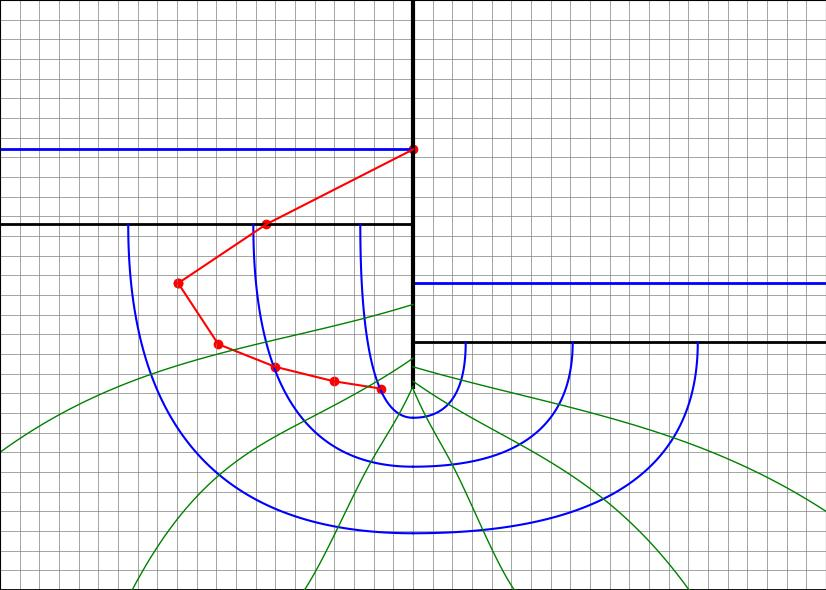
\includegraphics[width=\textwidth]{GRAFICOS/caso_2_presion_ataguia_neta.jpg}
        \caption{Caso 2 Presión ataguía neta}
        \text{Fuente: Elaboración propia}
        \label{fig:caso_2_presion_ataguia_neta}
    \end{minipage}
    \begin{minipage}{0.32\textwidth}
        \centering
        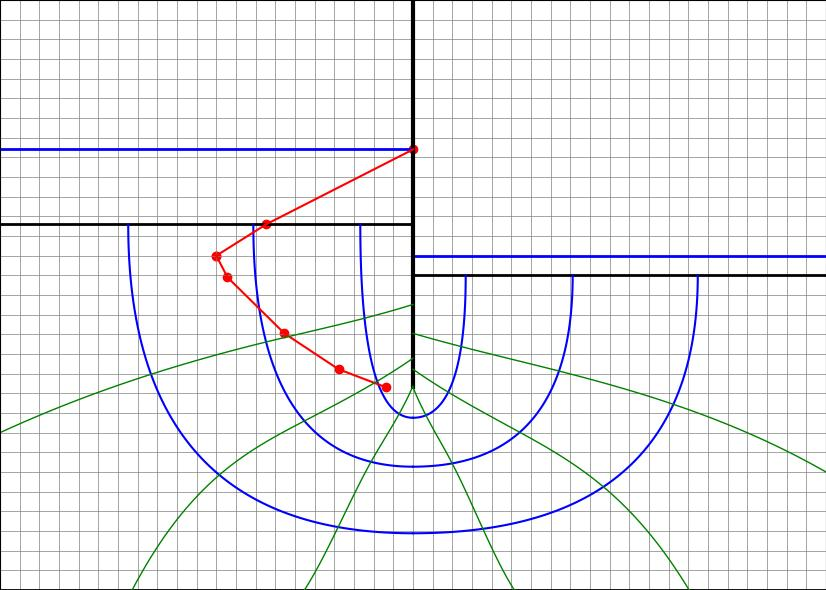
\includegraphics[width=\textwidth]{GRAFICOS/caso_3_presion_ataguia_neta.jpg}
        \caption{Caso 3 Presión ataguía neta}
        \text{Fuente:Elaboración propia}
        \label{fig:caso_3_presion_ataguia_neta}
    \end{minipage}
\end{figure}

Como se puede observar, a medida que el nivel del suelo sube, la presión en el fondo de la ataguía disminuye, lo que se traduce en una reducción de la presión efectiva. Esto se evidencia claramente en la figura \ref{fig:figura_11}, donde la presión efectiva es mayor en la parte inferior de la ataguía, mientras que, en la figura \ref{fig:figura_13}, los valores son menores.


\subsubsection{Estabilidad}
Finalmente, para determinar la estabilidad de la ataguía, se calculó el centroide de la ataguía en cada caso, basado en las presiones efectivas calculadas anteriormente.

\begin{figure}[H]
    \centering
    \begin{minipage}{0.32\textwidth}
        \centering
        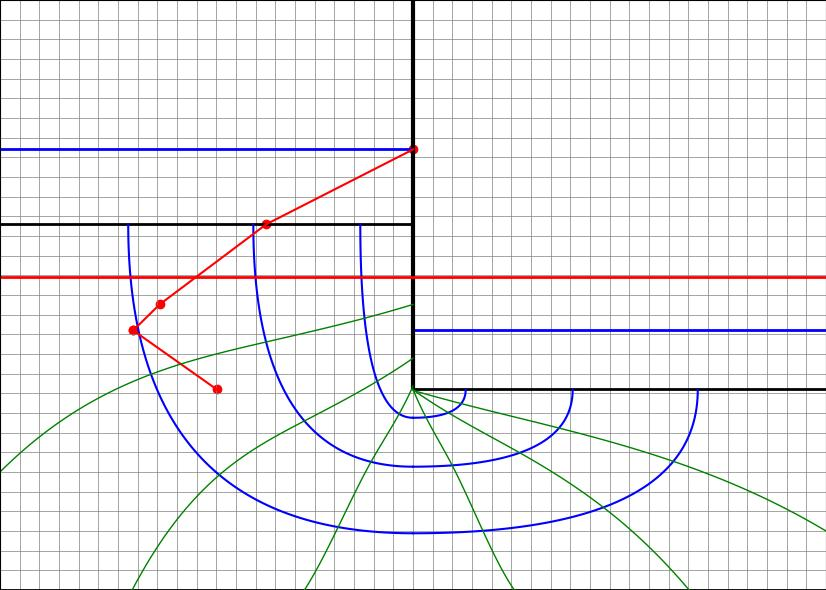
\includegraphics[width=\textwidth]{GRAFICOS/caso_1_centroide_y.jpg}
        \caption{Caso 1 Centroide}
        \text{Fuente: Elaboración propia}
        \label{fig:caso_1_centroide_y}
    \end{minipage}
    \begin{minipage}{0.32\textwidth}
        \centering
        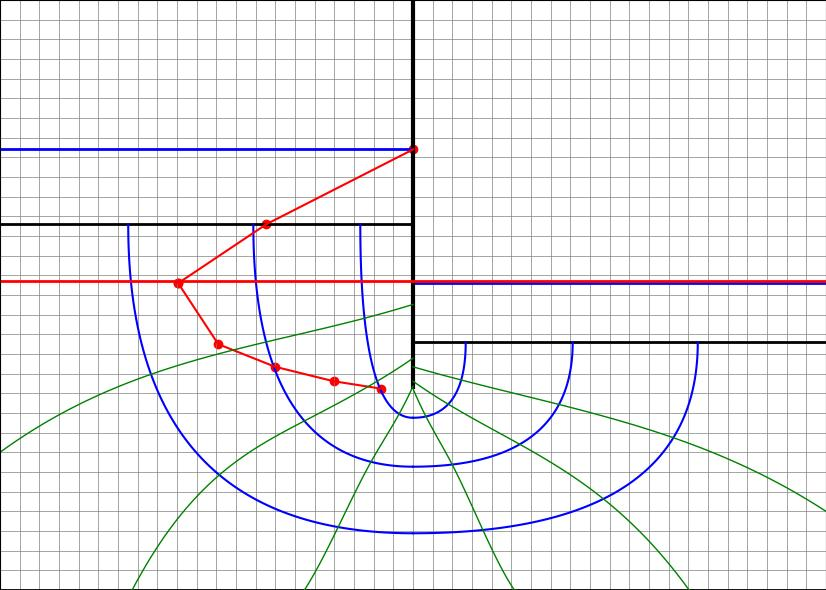
\includegraphics[width=\textwidth]{GRAFICOS/caso_2_centroide_y.jpg}
        \caption{Caso 2 Centroide}
        \text{Fuente: Elaboración propia}
        \label{fig:caso_2_centroide_y}
    \end{minipage}
    \begin{minipage}{0.32\textwidth}
        \centering
        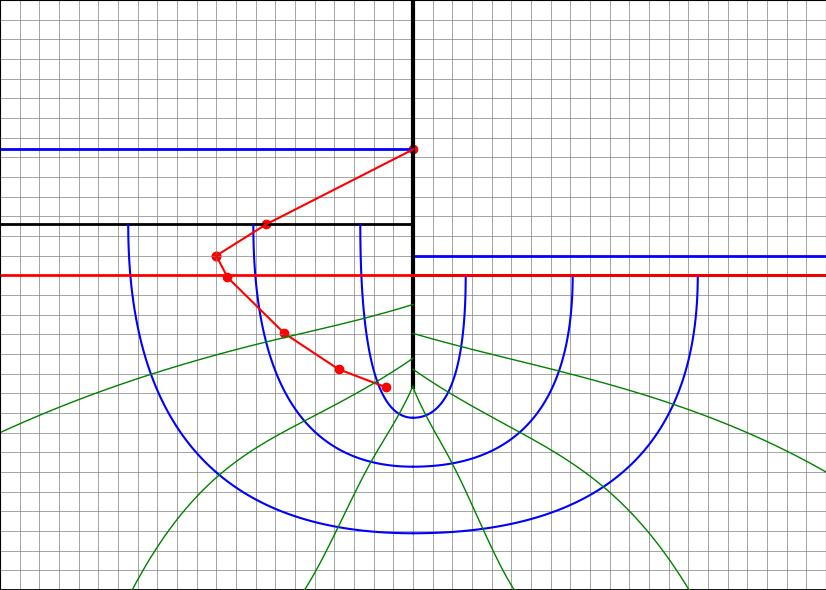
\includegraphics[width=\textwidth]{GRAFICOS/caso_3_centroide_y.jpg}
        \caption{Caso 3 Centroide}
        \text{Fuente: Elaboración propia}
        \label{fig:caso_3_centroide_y}
    \end{minipage}
\end{figure}

Como se puede observar, en la figura \ref{fig:caso_1_centroide_y}, el centroide se encuentra en una parte elevada de la ataguía. Esto produce un momento que tiende a voltear la ataguía, lo que conlleva a una menor estabilidad. Luego, a medida que el nivel de agua y suelo aumenta, el centroide se desplaza hacia abajo, lo que conlleva una mayor estabilidad y seguridad. 

\section{Análisis de Resultados}

Luego de aplicar los cálculos expresados en la sección de teoría, se obtuvieron los siguientes resultados para cada caso:

\begin{table}[H]
    \begin{center}
        \caption{Gradientes hidráulicos y caudales obtenidos manualmente.}
        \begin{tabularx}{0.75\textwidth}{>{\centering\arraybackslash}X >{\centering\arraybackslash}X >{\centering\arraybackslash}X >{\centering\arraybackslash}X >{\centering\arraybackslash}X}
        \hline
        \textbf{Propiedades} & \textbf{Caso 1} & \textbf{Caso 2} & \textbf{Caso 3} & \textbf{Unidades} \\
        \hline
        $i_{max}$ & $1.095$ & $0.629$ & $0.380$ & $-$ \\
        $i_{crit}$ & $1.141$ & $1.141$ & $1.141$ & $-$ \\
        $FS$ & $1.041$ & $1.811$ & $2.999$ & $-$\\
        $Q_{inf}$ & $43.877$ & $32.431$ & $25.754$ & $[\frac{m^3}{\text{día}}]$\\
        $k$ & $6.9 \times 10^{-5}$ & $6.9 \times 10^{-5}$ & $6.9 \times 10^{-5}$ & $[\frac{m}{s}]$\\
        \hline
        \end{tabularx}
        \label{tab:Manuales1}
        \text{Fuente: Elaboración propia}
    \end{center}
\end{table}

Los resultados obtenidos muestran que el gradiente hidráulico máximo ($i_{max}$) disminuye en cada caso, lo que sugiere una reducción en el flujo de agua alrededor de la ataguía, mientras que el gradiente crítico ($i_{crit}$) permanece constante en $1.141$, lo que indica que las propiedades del suelo no cambian. El factor de seguridad (FS) mejora notablemente en los casos 2 y 3, aumentando de $1.041$ en el primer caso a $2.999$ en el tercer caso, lo que sugiere una mayor estabilidad a medida que se reducen los gradientes. El caudal de infiltración ($Q_{inf}$) también disminuye de $43.877 \ \frac{m^3}{\text{día}}$ en el primer caso a $25.754 \ \frac{m^3}{\text{día}}$ en el tercer caso, lo que indica un mejor control del flujo de agua. Finalmente, el coeficiente de permeabilidad ($k$) se mantiene constante en $6.9 \times 10^{-5} \ \frac{m}{s}$, debido a que las propiedades del suelo no varían entre los casos.

\section{Fuentes de error}

Al realizar los cálculos manualmente, existe la posibilidad de cometer errores humanos durante las operaciones matemáticas, lo cual puede impactar la precisión de los resultados. Asimismo, la interpretación de los diagramas de flujo y equipotenciales puede ser subjetiva, generando posibles inexactitudes en la estimación de las propiedades del suelo. Por otra parte, trabajar con un número reducido de líneas equipotenciales y de flujo podría omitir detalles importantes del comportamiento del agua alrededor de la ataguía, afectando así la precisión de los cálculos.

